\chapter{Gate Array Partial Reconfiguration}
\label{cap5}
Le FPGA oltre la loro riprogrammazione, già vista nel capitolo precedente, si rendono ancora più versatili tramite l'uso delle regioni, esse rappresentano una parte di FPGA che può esser riprogrammata senza intaccare il resto della board, questo permette di avere molteplici acceleratori.\\
Le regioni definite nel seguente modo
\begin{figure}
    \centering
    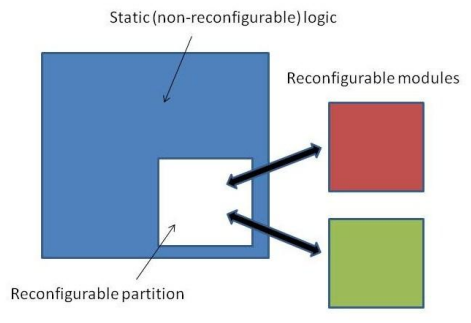
\includegraphics[width=0.4\textwidth]{images/PR1.png}
    \caption{Definizione regioni FPGA}
    \label{fig:my_label}
\end{figure}\\
Non tutte le regioni però sono riprogrammabili, ma solo alcune che vengono dette \textit{Partially Reconfigurable Region} (PRR). Questo modo di definire le FPGA rende ancora più conveniente la loro integrazione in un sistema IoT-Cloud.
\section{Place and Route per il Partial Bitstream}
La creazione di un Partial Bitstream, parte prima dalla progettazione dell'hardware, dove dovremmo descrivere, tramite Verilog o VHDL, un Intellectual Property(IP)\cite{PRRGIT}, un soft core che sia una blackbox, tramite essa sarà possibile effettuare il \textit{floorplanning}, esso è un tentativo di rappresentazione di come saranno piazzati i blocchi funzionali.
\begin{figure}
    \centering
    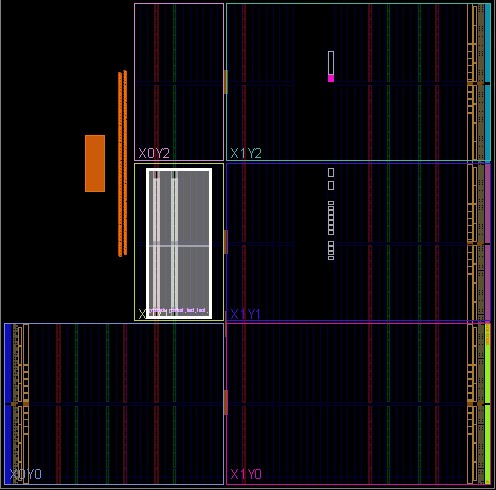
\includegraphics[width=0.4\textwidth]{images/Floor1.jpg}
    \caption{FloorPlanning in un FPGA Xilinx}
    \label{fig:my_label}
\end{figure}\\
Effettuato ciò potremmo effettuare il \textit{Place and Route}, generando cosi l'implementazione della scheda al fine di generare il \textit{Bitstream}\cite{PRR}. 
\section{Interfaccia per la riprogrammazione}
Le FPGA SoC permettono la programmazione della Programmable Logic tramite il Processing System, esso si interfaccerà tramite l'interfaccia \textit{Device Configuration interface}(DevC), essa possiede un'interfaccia DMA che tramite il bus AXI trasferirà il partial bitstream ad una delle due \textit{Configuration Access Port}, rispettivamente \textit{Processor Configuration Access Port}(PCAP) e \textit{Internal Configuration Access Port} (ICAP).
\begin{figure}
    \centering
    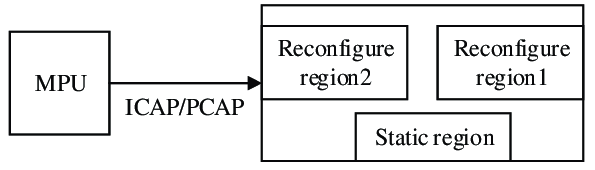
\includegraphics[width=0.4\textwidth]{images/PRR.png}
    \caption{Esempio di interfacciamento tra PS e PL per la riprogrammazione\cite{PRR2}}
    \label{fig:my_label}
\end{figure}\\
La loro coesistenza non è permessa dall'architettura, è possibile lo scambio tra le due interfacce anche runtime, tramite la modifica di un registro interno alla Processing System.\\
La Xilinix garantisce un IP core \textit{AXI$\_$HWICAP}, che abilita la \textit{Partial Reconfiguration} tramite l'uso di \textit{ICAP}. Il processo di riprogrammazione parziale è stato svolto tramite l'uso di un controller chiamato \textit{ZyCap}\cite{PRR}
\begin{figure}
    \centering
    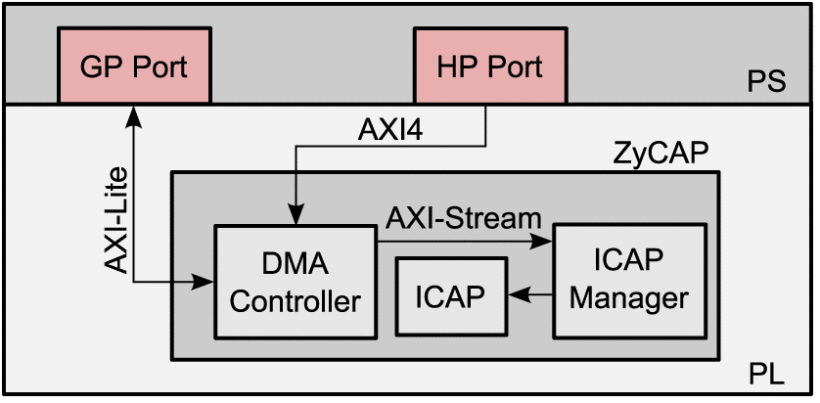
\includegraphics[width=0.4\textwidth]{images/ZyCap.png}
    \caption{Interfaccia tra PS e PL con il controller}
    \label{fig:my_label}
\end{figure}\\
\section{Problemi e possibili soluzioni}
Sfortunatamente l'architettura scelta al fine della realizzazione della tesi non supportava nativamente la \textit{Partial Reconfiguration}, rendendo impossibile la realizzazione di quest'ultima, anche causa un'obsoleta letteratura scientifica.\\
Il principale problema è dovuto dalla non completa integrazione di vivado con i meccanismi di sviluppo dei partial bitstream, poichè risulta impossibile esportare la definizione del hardware contenente tutte le informazioni inerenti al FPGA appena progettata, qualora si riuscisse ad esportare il file XSA sarà necessario creare il progetto su Vitis, ma le librerie usate in \cite{PRR} sono buona parte deprecate, rendendo inutile il processo di progettazione del codice per la riprogrammazione.\\
\subsection{Possibili soluzioni}
Alcuni possibili soluzioni potrebbero essere il cambio di architettura come ad esempio il passaggio a \textit{ZynqMP}, ma anche la creazione di un nuovo controller sulla base del \textit{Zycap}, quindi usando un \textit{AXI DMA} ed un controller per gli \textit{ICAP}. Ovviamente la creazione di un nuovo controller comporta la riscrittura del driver di riprogrammazione, che per alcuni tratti può esser basato su quello usato per il controllo del bus AXI, il driver dovrà necessariamente interfacciarsi con l'interfaccia \textit{DevC}, la quale però viene astratta tramite una libreria già fornita dalla Xilinix.\\
Il metodo appena descritto può esser usato per effettuare una riprogrammazione BareMetal, quindi senza la presenza di un sistema operativo lato PS, questo comporta l'introduzione di un elemento in più, assimilabile ad un raspberry, che ospiterà l'agente Lightning-rod per la connessione al cloud.


